\let\negmedspace\undefined
\let\negthickspace\undefined
\documentclass[journal]{IEEEtran}
\usepackage[a5paper, margin=10mm, onecolumn]{geometry}
%\usepackage{lmodern} % Ensure lmodern is loaded for pdflatex
\usepackage{tfrupee} % Include tfrupee package

\setlength{\headheight}{1cm} % Set the height of the header box
\setlength{\headsep}{0mm}     % Set the distance between the header box and the top of the text

\usepackage{gvv-book}
\usepackage{gvv}
\usepackage{cite}
\usepackage{amsmath,amssymb,amsfonts,amsthm}
\usepackage{algorithmic}
\usepackage{graphicx}
\usepackage{textcomp}
\usepackage{xcolor}
\usepackage{txfonts}
\usepackage{listings}
\usepackage{enumitem}
\usepackage{mathtools}
\usepackage{gensymb}
\usepackage{comment}
\usepackage[breaklinks=true]{hyperref}
\usepackage{tkz-euclide} 
\usepackage{listings}
% \usepackage{gvv}                                        
\def\inputGnumericTable{}                                 
\usepackage[latin1]{inputenc}                                
\usepackage{color}                                            
\usepackage{array}                                            
\usepackage{longtable}                                       
\usepackage{calc}                                             
\usepackage{multirow}                                         
\usepackage{hhline}                                           
\usepackage{ifthen}                                           
\usepackage{lscape}
\begin{document}

\bibliographystyle{IEEEtran}
\vspace{3cm}




\title{
%	\logo{
GATE - 2009 - XE

\large{EE1030 : Matrix Theory}

Indian Institute of Technology Hyderabad
%	}
}
\author{Satyanarayana Gajjarapu

AI24BTECH11009
}	





\maketitle




\bigskip

\renewcommand{\thefigure}{\theenumi}
\renewcommand{\thetable}{\theenumi}


\section{13 - 24}


\begin{enumerate}
\item Under what conditions is the equation $\Delta \cdot \rho \overrightarrow{V} = 0$ valid ?\\
P : Steady incompressible flow \\
Q : Unsteady incompressible flow \\
R : Steady compressible flow \\
S : Unsteady compressible flow 
    \begin{enumerate}
        \item P,Q,R
        \item Q,R,S
        \item P,R,S
        \item P,Q,S \\
    \end{enumerate}
\item Stream function CANNOT be defined for
\begin{enumerate}
    \item two dimensional incompressible flow
    \item two dimensional compressible flow
    \item three dimensional incompressible flow
    \item axisymmetric incompressible flow \\
\end{enumerate}
\item Which one of the following is an irrotational flow ?
\begin{enumerate}
    \item Free vortex flow
    \item Forced vortex flow
    \item Couette flow
    \item Wake flow \\
\end{enumerate}
\item Under strong wind conditions, electrical cables can be subjected to wind-induced oscillations. Which one of the following non-dimensional numbersis relevant to this problem ?
 \begin{enumerate}
     \item Froude number
     \item Weber number
     \item Faraday number
     \item Strouhal number \\
 \end{enumerate}
\item Dimples are made on golf balls for which of the following reasons ? \\
P : to make the ball travel a longer distance \\
Q : to make the flow over the ball turbulent \\
R : to make the flow over the ball laminar \\
S : to create a separated boundary layer flow over the ball
\begin{enumerate}
    \item P, Q
    \item Q, S
    \item R, S
    \item P, R \\
\end{enumerate}
\item In a 2-D boundary layer flow, $x$ and $y$ are the streamwise and wall-normal coordinates, respectively. If $u$ denotes the velocity along $x$ direction, which one of the following represents the condition at the point of flow separation ?
\begin{enumerate}
    \item $\frac{\partial u}{\partial x} = 0$
    \item $\frac{\partial u}{\partial y} = 0$
    \item $\frac{\partial^2 u}{\partial x^2} = 0$
    \item $\frac{\partial^2 u}{\partial y^2} = 0$ \\
\end{enumerate}
\item Which one among the following boundary layer flows is the LEAST susceptible to flow separation ?
\begin{enumerate}
    \item turbulent boundary layer in a favourable pressure gradient
    \item laminar boundary layer in a favourable pressure gradient
    \item turbulent boundary layer in an adverse pressure gradient
    \item laminar boundary layer in an adverse pressure gradient \\
\end{enumerate}
\item Air from the blower of a hairdryer flows between two identical elliptical cylinders suspended freely, for two cases shown in the figure. The cylinders would move 
\begin{figure}[!ht]
\centering
\resizebox{0.5\textwidth}{!}{%
\begin{tabular}{|c|c|c|c|c|}
\hline
$x$ & $x_1 = 2$ & $x_2 = 6$ & $x_3 = 8$ & $x_4 = 9$ \\
\hline
$f$ & $4$ & $4$ & $\alpha$ & $\beta$ \\
\hline
\end{tabular}


}%
\end{figure}
 \begin{enumerate}
    \item away from each other for Case 1 and towards each other for Case 2
    \item towards each other for Case 1 and away from each other for Case 2
    \item away from each other for Case 1 and away from each other for Case 2
    \item towards each other for Case 1 and towards each other for Case 2 \\
 \end{enumerate}
\item A 40 cm cubical block slides on oil (viscosity = 0.80 Pa.s), over a large plane horizontal surface. If the oil film between the block and the surface has a uniform thickness of 0.4 mm, what will be the force required to drag the block at 4 m/s ? Ignore the end effects and treat the flow as two dimensional.
\begin{enumerate}
     \item 1280 N
     \item 1640 N
     \item 1920 N
     \item 2560 N \\
 \end{enumerate}
\item For a floating body, G, B, and M represent centre of gravity, centre of buoyancy, and the metacentre, respectively. The body will be stable if
\begin{enumerate}
    \item G is located above B
    \item B is located above M
    \item M is located above B
    \item M is located above G \\
\end{enumerate}
\item A nozzle has inlet and outlet diameters of 10 cm and 5 cm, respectively. If it discharges air at a steady rate of 0.1 $\text{m}^3$/s into atmosphere, the gauge pressure (static) at the nozzle inlet will be
\begin{enumerate}
    \item 1.26 kPa
    \item 1.46 kPa
    \item 3.52 kPa
    \item 3.92 kPa \\
\end{enumerate}
\item Consider incompressible flow through a two-dimensional open channel. At a certain section A-A, the velocity profile is parabolic. Neglecting air resistance at the free surface, find the volume flow rate per unit width of the channel.
 \begin{figure}[h!]
	    \centering
	    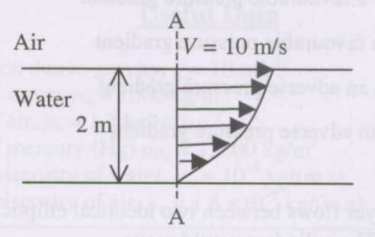
\includegraphics[width=0.5\linewidth]{figs/Q12.png}
	      \end{figure}
 \begin{enumerate}
    \item 10 $\text{m}^3$/s
    \item 13.33 $\text{m}^3$/s
    \item 20 $\text{m}^3$/s
    \item 33.33 $\text{m}^3$/s \\
\end{enumerate}
			 \end{enumerate}
			 \end{document}
 
